\documentclass{article}
\usepackage{polski}
\usepackage[utf8]{inputenc}
\usepackage{latexsym}
\usepackage{graphicx} 
\usepackage{float}
\begin{document}
	
	\title {Politechnika Poznańska \\Lokalizator użytkowników sieci WiFi }
	\maketitle
	\begin{tabular}{|r|l|l|} \hline
		Maciej Michalak & 121992 & maciej.k.michalak@student.put.poznan.pl \\
			\hline
		Patryk Masiakowski & 116285 & patryk.masiakowski@student.put.poznan.pl \\
			\hline
		Jakub Kostrzewski & 122039 & jakub.k.kostrzewski@student.put.poznan.pl \\
		\hline
	\end{tabular}
\newpage
\tableofcontents
\newpage
\listoffigures
\newpage
\section{Wstęp}
\subsection{Opis aplikacji}
Celem projektu jest stworzenie aplikacji pozwalającej na określenie lokalizacji użytkownika sieci względem trzech urządzeń AP. System powinien przeskanować sieć w poszukiwaniu klientów podłączonych do punktów dostępowych. Użytkownik będzie mieć możliwość podejrzenia podstawowych informacji o każdym hoście w sieci, takicj jak nr. ip czy adres MAC. Do określenia względnej lokalizacji w sieci wykorzystana zostanie technika trilateracji. Aplikacja działa na zasadzie serwera interpretującego dane przesłane przez punkty dostępowe. Klienci powinni znaleść w swoim otoczeniu trzy punkty dostępowe, które mają wzlędem nich określoną siłę syganłu. Dane o tych sygnałach zostają przesyłane do serwera i interpretowane. W czasie rzeczywiśtym podawana jest lokalizacja danego klienta. 


\section{Działanie}

\subsection{Trilateracja}
Jest to metoda określania położenia obiektu w trójwymiarowej przestrzeni(w tym wypadku budynku). By metoda ta była skuteczna wymagana jest znajomość położenia trzech punktów dostępowych (AP).Znająć odległości każdego punktu dostępowego od lokalizowanego urządzenia oraz współrzędne tych punktów można określić lokalizację urządzenia. 



Każdą odległość AP od lokalizowanego urządzenia można przedstawić w przestrzeni jako sfere. Wyznaczenie współrzędnych klienta sprowadza się do znaleznienia miajsca przecięcia trzech sfer, każdej związanej z AP.


\begin{figure}[H]
	\centering
	\includegraphics[width=6cm]s
	\caption{Sfery wyznaczone przez siłe sygnału AP}
	\label{fig:obrazek s.jpg}
\end{figure}

\begin{figure}[H]
	\centering
	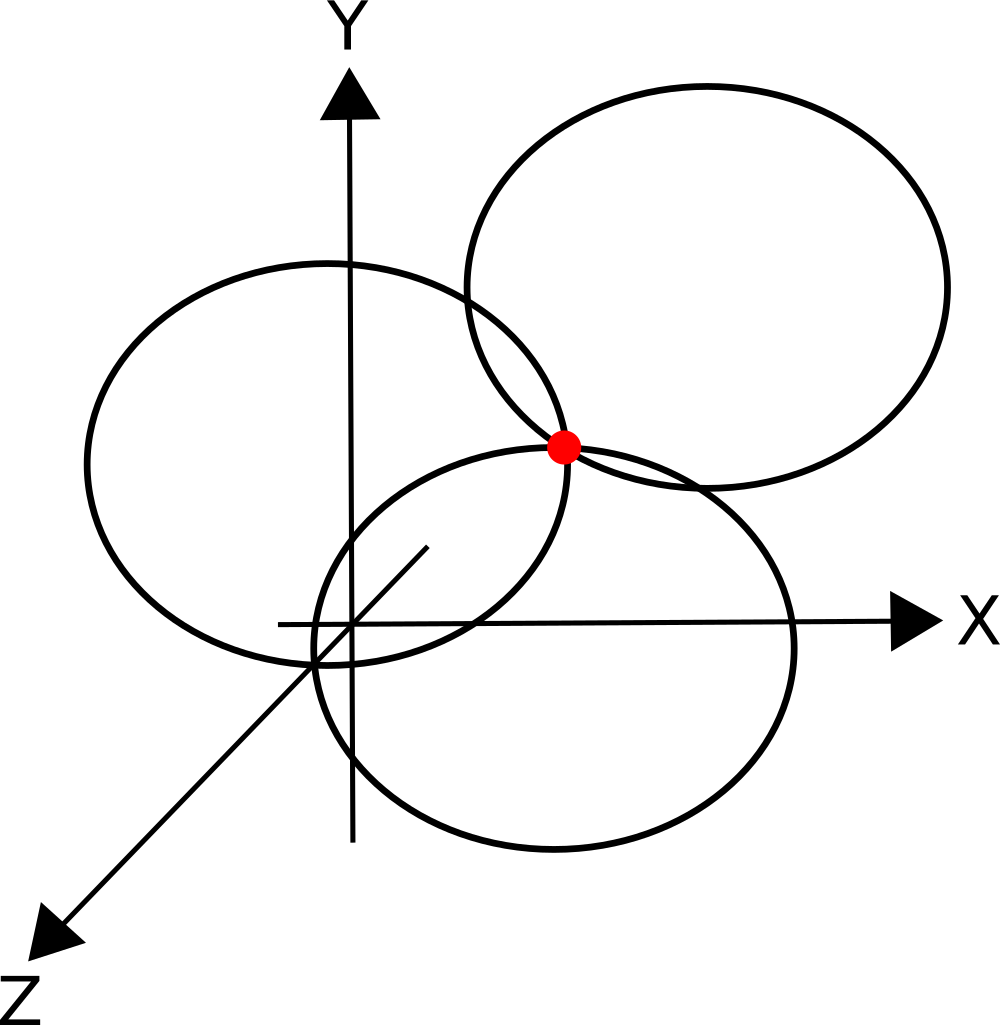
\includegraphics[width=4cm]{3d-os.png}
	\caption{Siła sygnału w przestrzeni}
	\label{fig:obrazek 3d-os.png}
\end{figure}


\subsection{SSID i BSSID}

Początkowym etapem działania aplikacji będzie lokalizowanie pobliskich punktów dostępowych i ich identyfikacja na podstawie 48-bitowego numeru identyfikacyjnego BSSID czyli numeru MAC AP oraz identyfikatora SSID.


\begin{figure}[H]
	\centering
	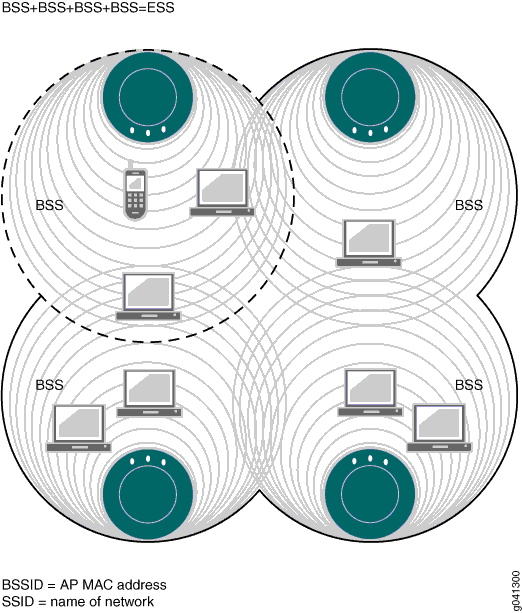
\includegraphics[width=8cm]{bssid.png}
	\caption{BSSID i ESSID}
	\label{fig:obrazek bssid.png}
	\end{figure}




\begin{figure}[H]
	\centering
	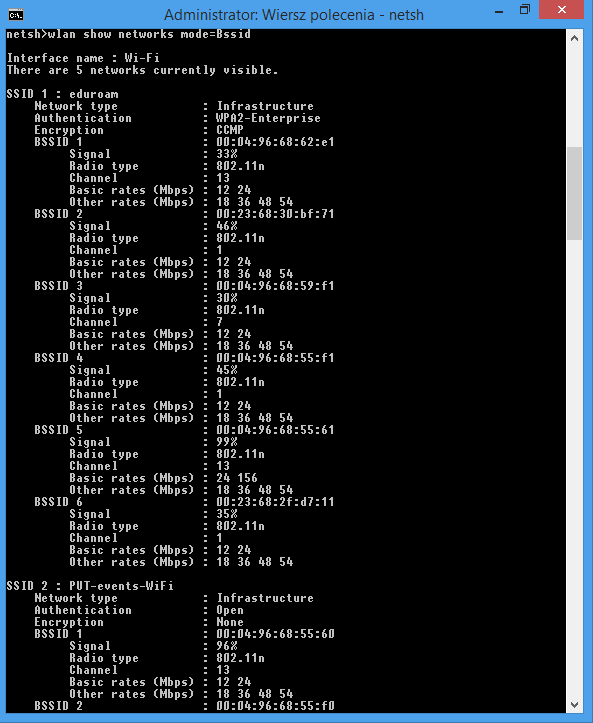
\includegraphics[width=10cm]{przykladbssid.png}
	\caption{Listowanie dostępnych essid}
	\label{fig:obrazek przykladbssid.png}
\end{figure}



\subsection{RSSI}

RSSI jest wskażnikiem mocy sygnału nadawanego przez dany punkt dostępowy. Wykorzystując wartości tego wskaźnika, możliwe jest określenie odległości lokalizowanego urządzenia od punktu dostępowego.



\subsection{Punkty dostępowe}

Do przeprowadzenia testów aplikacji zostanie "zbudowana" prosta sieć utworzona na hotspotach z telefonów komórkowych. Do poprawnego działania będą potrzebne trzy lub więcej punkty dostępowe.

\subsection{Beacony i ProbeRequest}

\textbf{Ramki Beacon} służą punktom dostępowym do informowania potencjalnych klientów sieci o świadczeniu usługi połączenia bezprzewodowego. Zawierają informacje o adresie fizycznym AP.
\newline
\newline
\textbf{Probe Request} to pakiety wysyłane przez urządzenia sieciowe(np. smartfony) w celu wykrycia dostępnych punktów dostępowych. AP po otrzymaniu takiego pakietu może odczytać jaka jest siła sygnału urządzenia klienta względem niego.

\subsection{Aplikacja serwera}

Serwer otrzymuje dane od klienta i na podstawie poniższego wzoru wyznacza odległości do trzech punktów dostępowych. Następnie rysuje sfery i podaje lokalizacje użytkownika (część wspólna sfer).
\newline
\newline
\Huge{
\begin{math}
d = 10 ^{((TxPower - RSSI) / (10 * n))}
\end{math}
}
\newline
\newline
\normalsize{
\textbf{d} - odległość w metrach \newline
\textbf{TxPower} - maksymalna siła sygnału AP \newline
\textbf{RSSI} - sygnał AP z punktu widzenia klienta \newline
\textbf{n} - stała propagacji(2 dla wolnych przestrzeni) \newline
}


\begin{figure}[H]
	\centering
	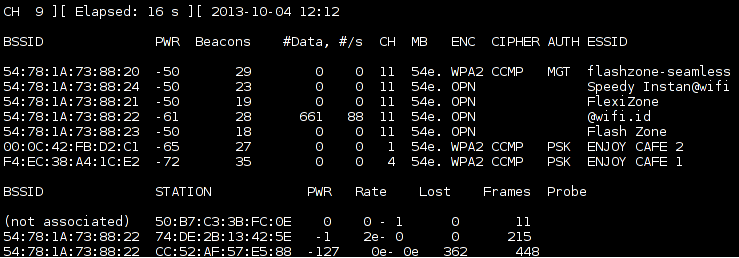
\includegraphics[width=15cm]{airodump.png}
	\caption{Przykładowe działanie airodump-ng}
	\label{fig:obrazek airodump.png}
\end{figure}

\newpage
\subsection{Harmonogram prac}
\begin{figure}[H]
	\centering
	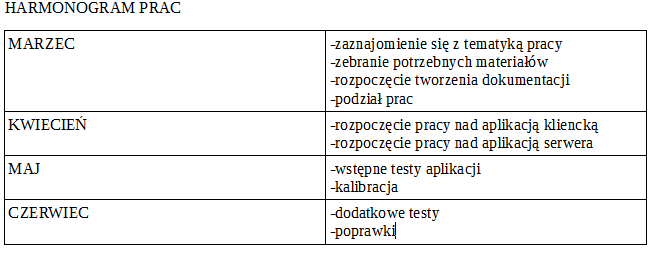
\includegraphics[width=15cm]{harmonogram.png}
	\caption{Harmonogram prac}
	\label{fig:rysowanie.png}
\end{figure}



\subsection{Funkcje-klient}


\begin{itemize}
\item wyszukiwanie dostępnych AP po BSSID,
\item pobieranie danych o sygnale względem każdego BSSID,
\item wysyłanie danych do serwera.
\end{itemize}

\subsection{Funkcje-serwer}


\begin{itemize}
	\item wyświetlanie dostępnych klientów w sieci,
	\item pobieranie danych o sygnałach RSSI od klientów,
	\item obliczanie lokalizacji w przestrzeni na podstawie trilateracji.
\end{itemize}
\newpage

\section{Symulowanie działania aplikacji klienta}

Z powodu problemów z odpowiednim odczytywaniem odległości punktów dostępowych, napisany został program symulujący wysyłanie "odpowiednich" dacnyh do serwera. Znaczy to w tym wypadku, że konkretna siła sygnału prezentuje zawsze tą samą odległości AP i wahania tych wartości nie są zbyt duże. Napisanie takiej aplikacji pozwoliło nam spreccyzować jaki efekt pracy chcemy uzyskać.


\section{Napotkane problemy i potenjclane problemy przy dalszym rozwoju aplikacji}

Mimo, że w teorii działanie aplikacji nie opiera się na żadnych skomplikowanych metodach czy obliczeniach, kilka rzeczy okazało się problematyczne. Projekty tego typu cieszą się raczaj wątpliwą popularnością i ciężko o udokumentowane przypadki naprawde dokładnego lokalizowania użytkownika sieci WiFi. Czymś co na pewno mogłoby uskutecznić działanie takiego systemu to możliwości finansowe. Pozwoliłoby to przygotować w pełni autorskie środowisko testowe.

Kwestiami problematycznymi w projekcie okazały sie:

\begin{itemize}
	\item \textbf{Sygnał RSSI nie jest dobrą miarą odległosci od AP} - siła sygnału punktu dostępowego może zależeć od wielu rzeczy. Mocy nadajnika, mocy odbirnika, poziomu naładowania baterii w takowych, modelu sprzętu, który służy w testowaniu. Podczas testów aplikacji okazało się, że w przypadku sprzętu róznych producentów, z różnymi kartami sieciowymi czy antenami, nie udało się uzyskać dokładnych wyników. Dwa urządzenia, znajdujące się w tej samej odległości od urządzenia z aplikacją kliencką, pokazywały na serwerze inne odległości. Znacząco inne.
	
	\item \textbf{Kalibracja} - aplikacja miała z założenia działać na zasadzie nakładania na plany budynków punktów dostepowych, rozmieszczania ich. Po rozmieszczeniu każdy z punktów, w czasie rzeczywistym, odbierał dane od aplikacji klienta i rysował okręgi zasięgów na planie. Należało w odpowiedni sposób skalibrować mapę z rzeczywistymi wymiarami np. pomieszczeń. Szukanie pewnego wspołczynnika skalującego metry na piksele okazało się dosyć problematyczne.
	
	
\end{itemize}


\newpage

\section{Diagramy aplikacji}
\subsection{Diagram przypadków użycia}
Poniżej znajduje się podstawowy diagram przypadków użycia aplikacji. Pokazuje wszystkie funkcjonalności które oferuję aplikacja kliencka oraz serwerowa, z podziałem na aktorów.


\begin{figure}[H]
	\centering
	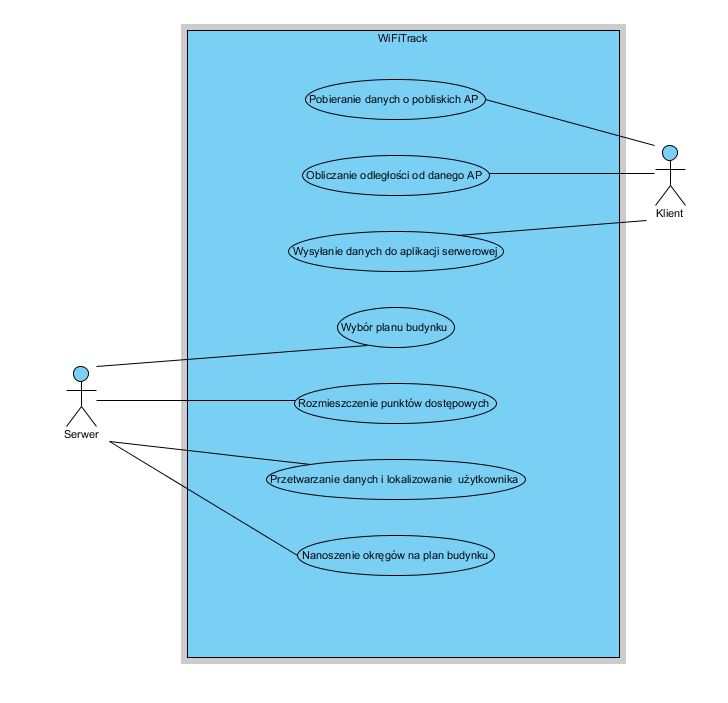
\includegraphics[width=15cm]{przypadkiuzycia.png}
	\caption{Diagram przypadkow użycia}
	\label{fig:przypadkiuzycia.png}
\end{figure}
\newpage
\subsection{Diagramy aktywności}
Diagram aktywności znajdujący się na rysunku poniżej przedstawia, jak przebiegają wszystkie procesy w naszym projekcie. Rozpoczynając od pobierania danych o punktach dostępowych z aplikacji klienckiej do rysowania okręgów odległości na ekranie aplikacji serwerowej.

\begin{figure}[H]
	\centering
	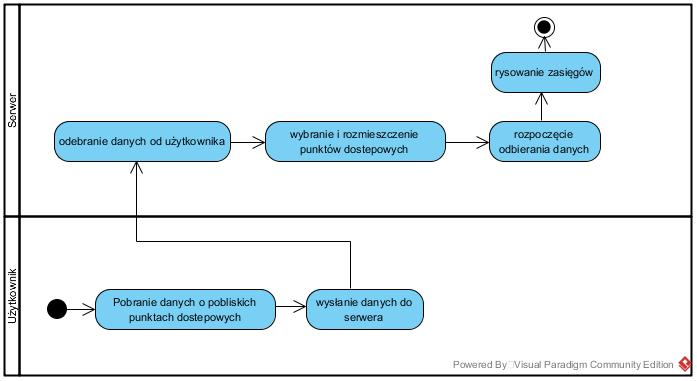
\includegraphics[width=15cm]{rysowanie.jpg}
	\caption{Diagram aktywności - rysowanie}
	\label{fig:rysowanie.jpg}
\end{figure}

\newpage
Kolejny diagram aktywności przedstawia działanie aplikacji klienckiej znajdującej się na urządzeniu moblinym. Diagram ukazuje kroki, które wykonuje aplikacja w tle. Wszystkie procesy oprócz zainicjowania wysyłania danych są wykonywane bez ingerencji klienta.

\begin{figure}[H]
	\centering
	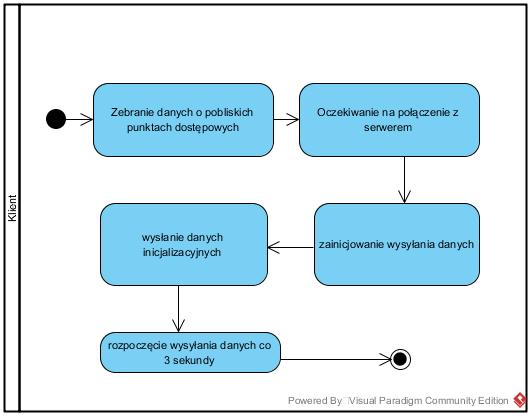
\includegraphics[width=10cm]{klient.jpg}
	\caption{Działanie apliakcji klienta}
	\label{fig:klient.jpg}
\end{figure}

\newpage

\section{Podstawowe mockupy aplikacji}

\subsection{Aplikacja serwerowa}

Widok aplikacji serwerowej zaraz po uruchomieniu programu. Mamy tutaj możliwość dostosowania naszej planszy(pomieszczenia), do powierzchni którą rzeczywiście zajmuję. Wymiary pomieszczenia podajemy w metrach. Po wpisaniu wymiarów wybieramy plik graficzny odzwierciedlający plany pomieszczenia lub budynku.

\begin{figure}[H]
	\centering
	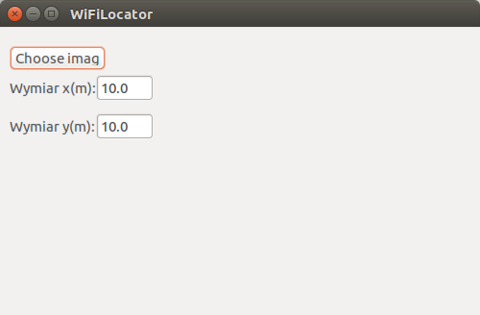
\includegraphics[width=15cm]{wymiary.png}
	\caption{Wybór wymiarów}
	\label{fig:rysowanie.jpg}
\end{figure}
\newpage
Widok aplikacji serwerowej w którym mamy możliwość ręcznego ustawienia położenia naszych AP za pomocą lewego przycisku myszy. Bardzo ważne jest żeby ustawić AP dokładnie, ponieważ od tego znacząco zależy dokładność naszej aplikacji.

\begin{figure}[H]
	\centering
	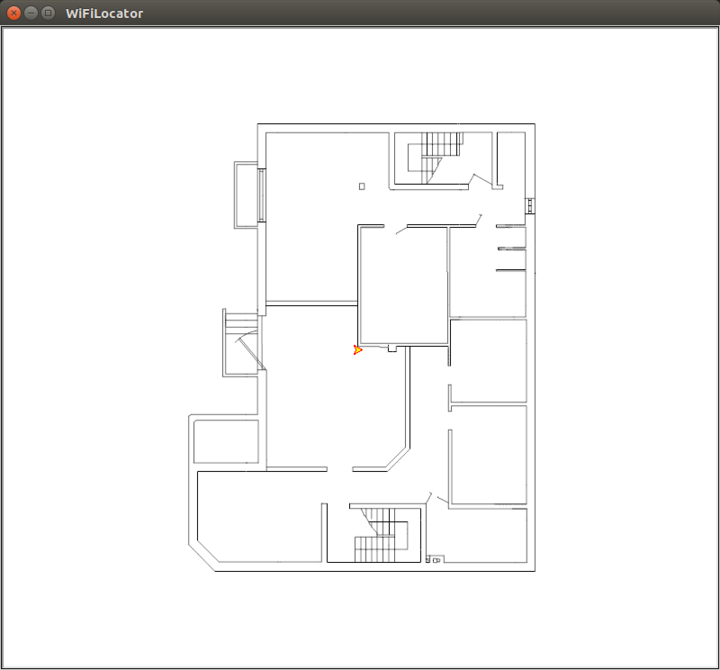
\includegraphics[width=15cm]{serwer.png}
	\caption{Aplikacja serwera po wybraniu pliku graficznego}
	\label{fig:rysowanie.jpg}
\end{figure}

\newpage
Ten widok aplikacji przedstawia przykładowe przesłane informacje z aplikacji klienckiej do aplikacji serwerowej. Pierwsze przesłanie danych skutkuje możliwością rozstawienia punktów dostepowych na wybranej przez nas wcześniej mapie. Kluczową kwestią w tym kroku jest dokładne rozstawienie punktów na planach budynku.

\begin{figure}[H]
	\centering
	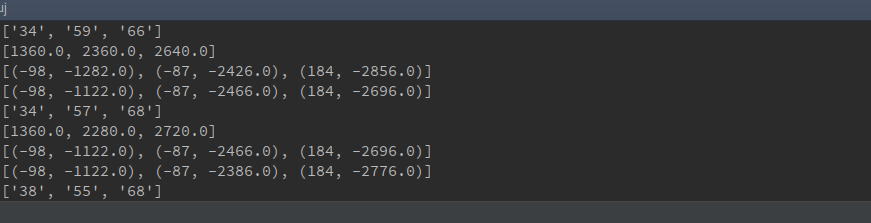
\includegraphics[width=15cm]{serwerDane.png}
	\caption{Przykładowe dane przesłane do aplikacji serwerowej}
	\label{fig:rysowanie.jpg}
\end{figure}
\newpage
Widok aplikacji poniżej przedstawia w pełni działającą aplikację serwerową. W tym miejscu następuje przesyłanie odległości klienta od zaznaczonych punktów dostepowych, które są odświeżane w odstępie czasowym 3 sekundy.
\begin{figure}[H]
	\centering
	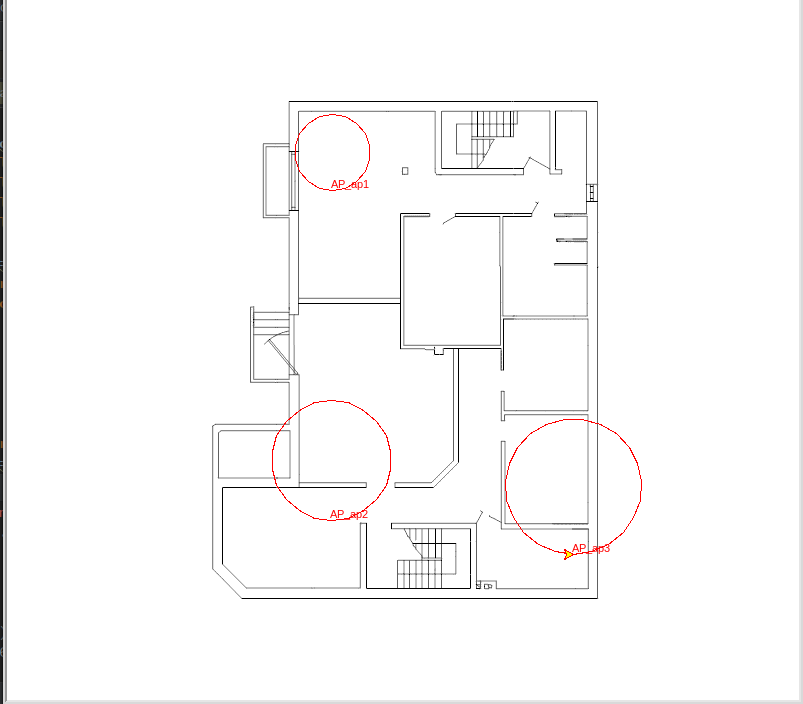
\includegraphics[width=15cm]{serwerKolo.png}
	\caption{Widok w pełni działającej aplikacji serwerowej}
	\label{fig:rysowanie.jpg}
\end{figure}
\newpage
\subsection{Aplikacja kliencka}
Widok okna aplikacji klienta pokazujący się gdy serwer nie jest aktualnie włączony. Aplikacja przejdzie do nowego okna widoku oraz rozpocznie przesyłanie danych zaraz po włączeniu serwera.
\begin{figure}[H]
	\centering
	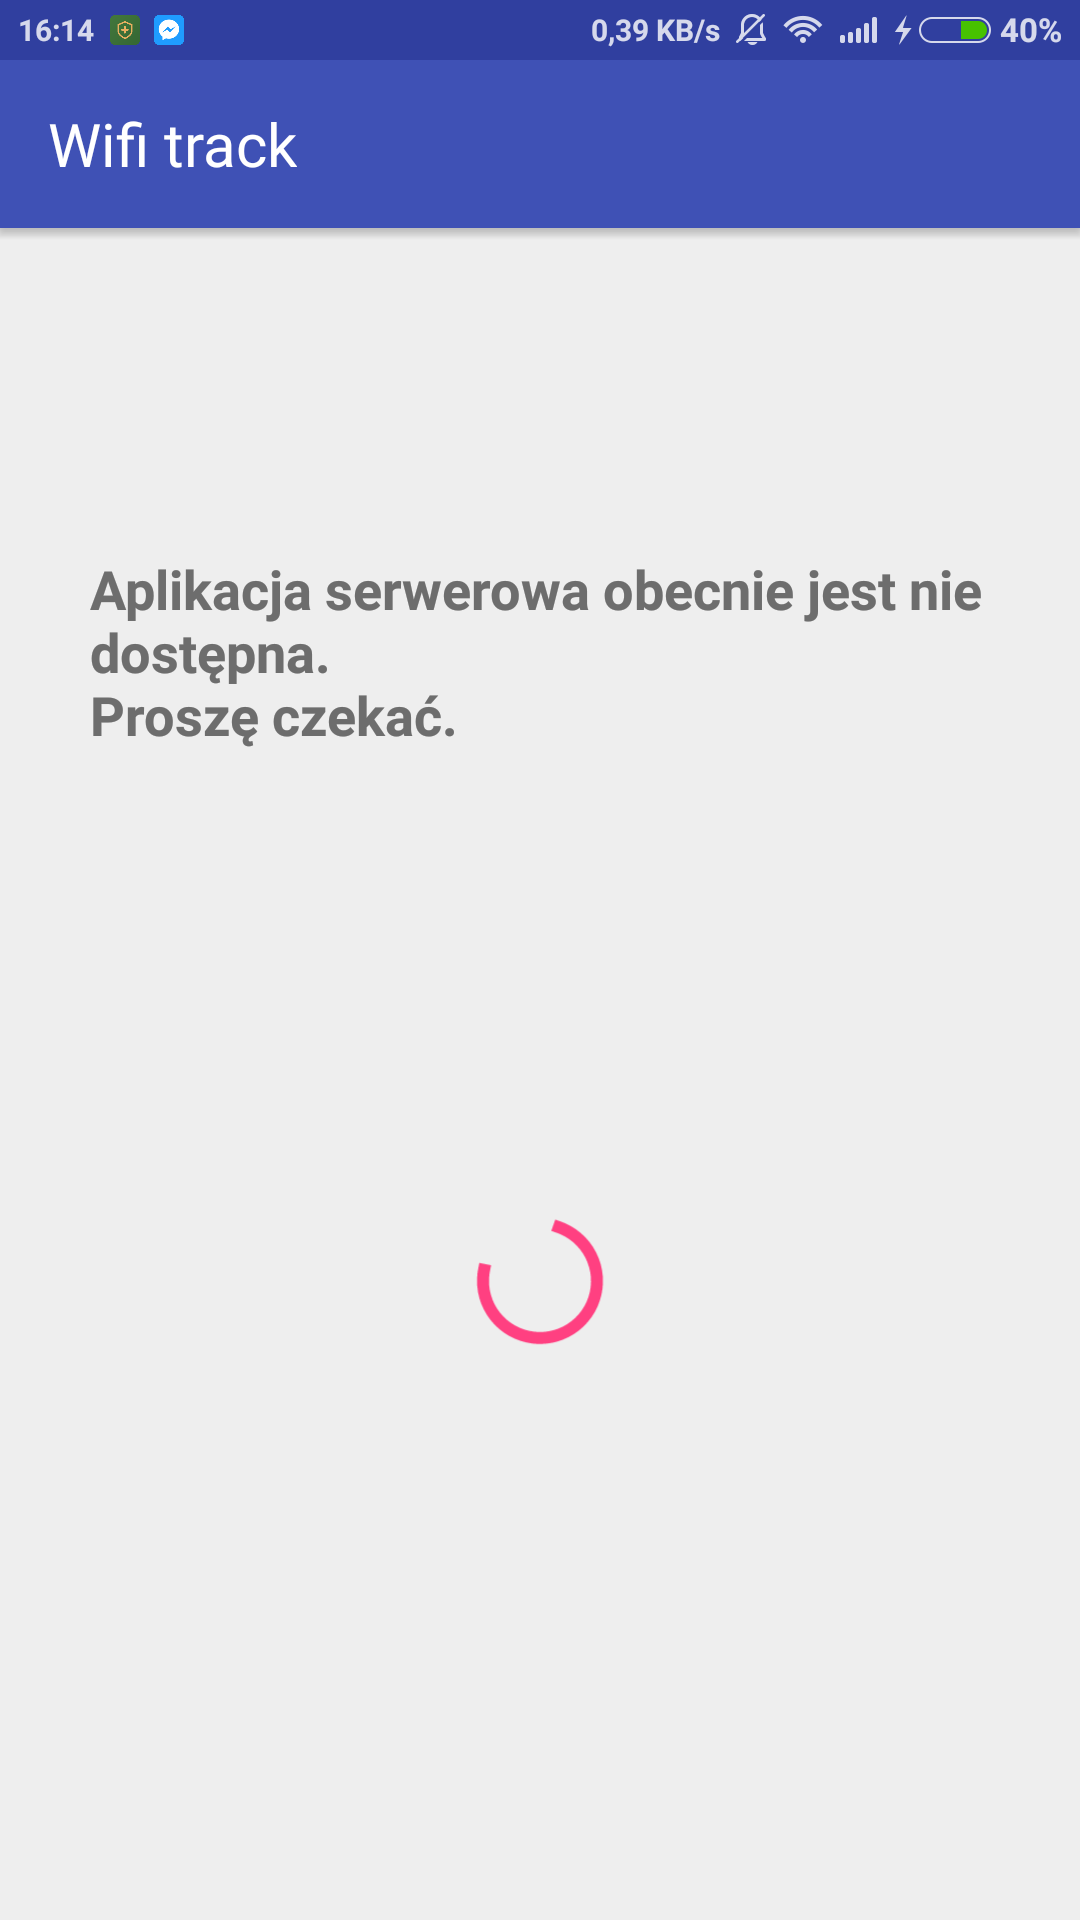
\includegraphics[width=9cm]{apkW8.png}
	\caption{Aplikacja czekająca na odpowiedź serwera}
	\label{fig:rysowanie.jpg}

\end{figure}
\newpage
Główny widok aplikacji klienta przedstawia listę AP z nazwami, dystansem, siłą signału, kanałem, częstotliwością oraz zabezpieczeniami. Po kliknięciu przycisku rozpoczęcia przesyłania danych wysyłane są wiadomości do serwera w odstępie czasowym 3 sekundy.
\begin{figure}[H]
	\centering
	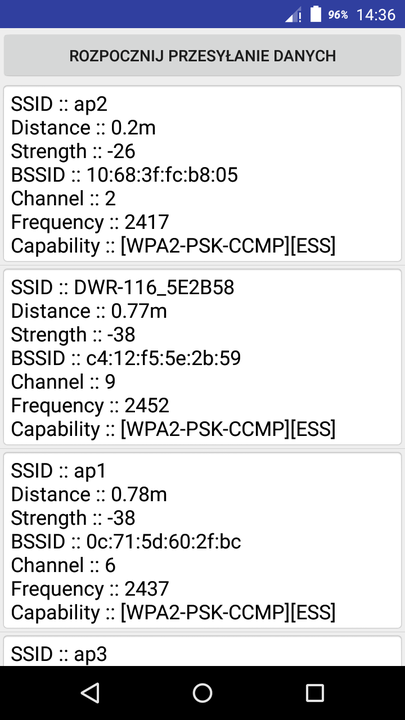
\includegraphics[width=9cm]{klient.png}
	\caption{Punkty dostępowe w apliakcji klienckiej}
	\label{fig:rysowanie.jpg}
\end{figure}

\newpage
Widok okna aplikacji klienta podczas obsługi błędu nagłej utraty połączenia z serwerem.
\begin{figure}[H]
	\centering
	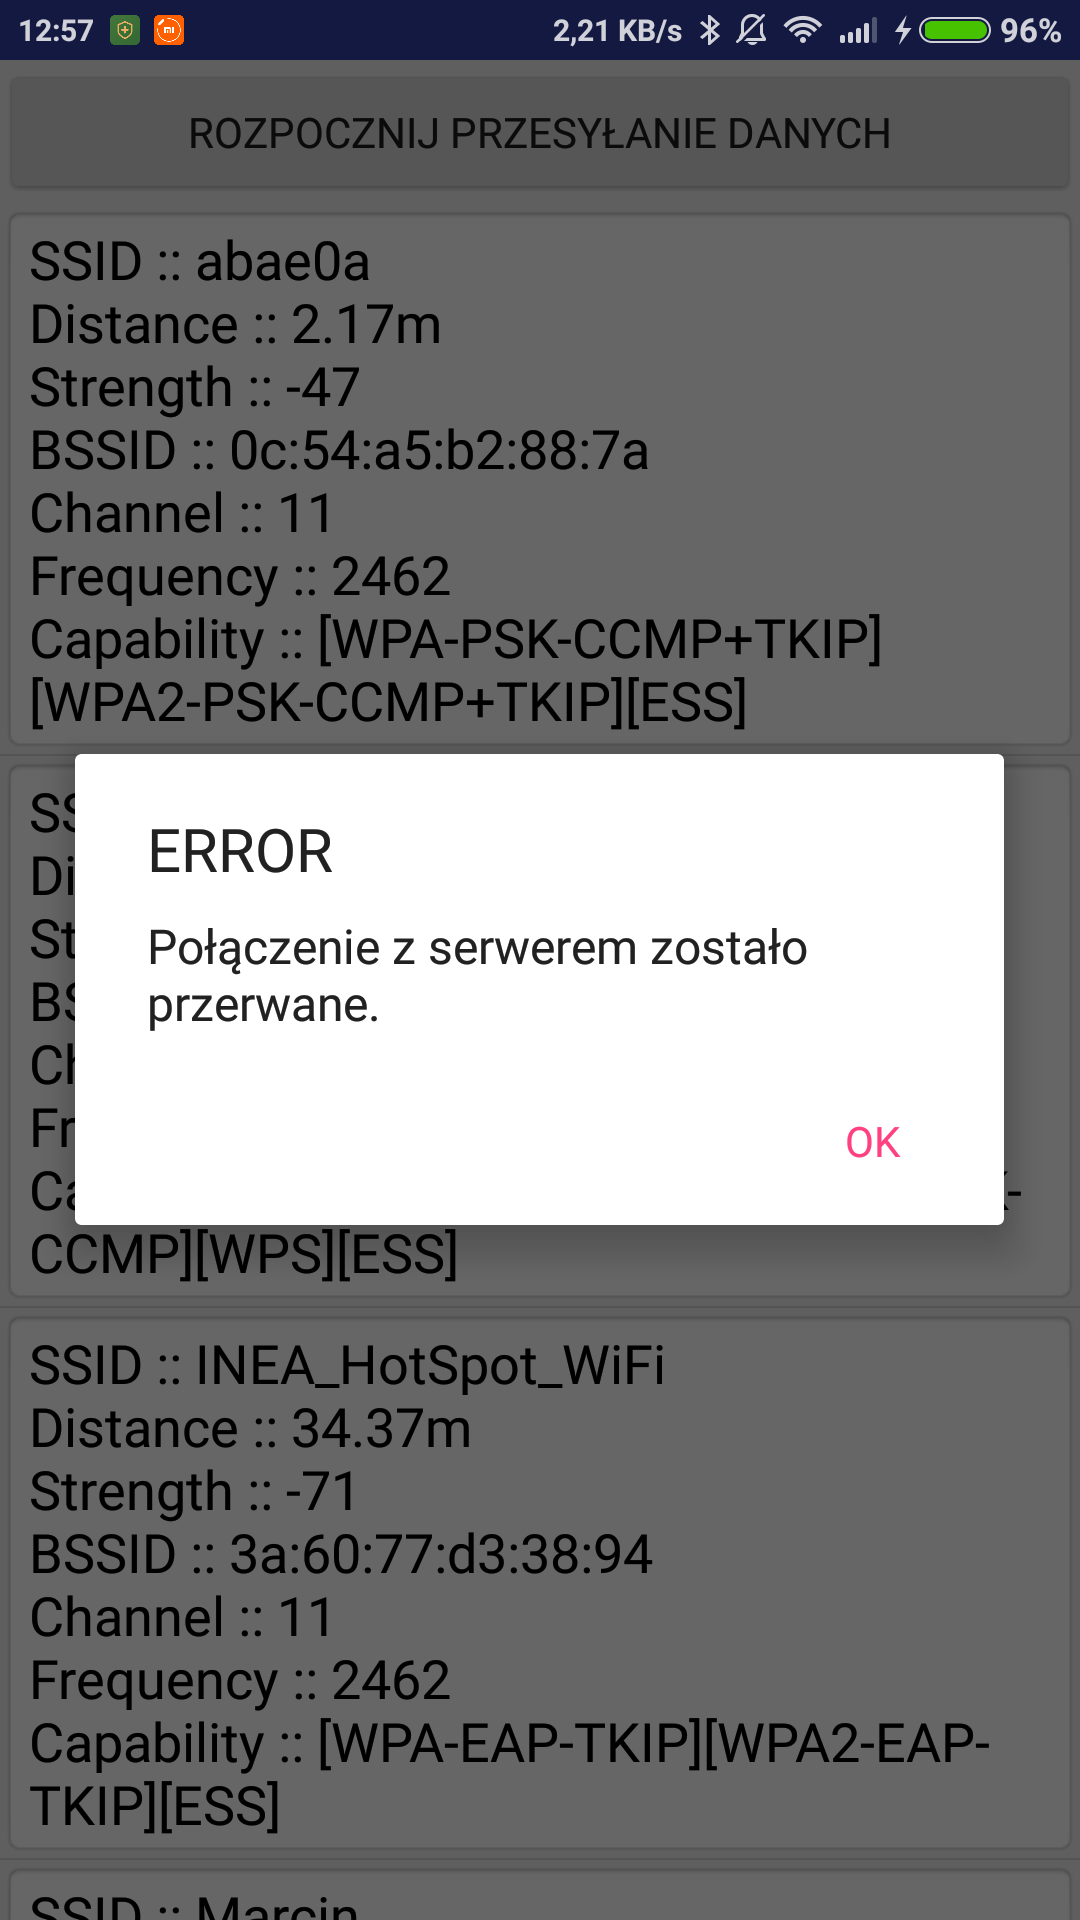
\includegraphics[width=9cm]{apkError.png}
	\caption{Okno błędu rozłączenia z serwerem}
	\label{fig:rysowani.jpg}
\end{figure}

\section{Możliwości rozwoju aplikacji}
\begin{itemize}
	\item \textbf{Podsumowanie odległości w czasie} - w przyszłości aplikacja mogłaby wyliczać odległość przebytą przez klienta na podstawie danych przesyłanych na serwer, w ten sposób moglibyśmy wyliczyć sume długości jaką klient przebył w trakcie miesiąca bądź roku.
	
	\item \textbf{Rysowanie tras} - do aplikacji klienckiej mógłby zostać dodany moduł który wyświetlałby narysowane przez serwer trasy po których się poruszaliśmy w trakcie naszego użytkowania aplikacji.
	
	\item \textbf{Obliczanie prędkości} - w aplikacji klienckiej w przyszłości moglibyśmy zaimplementować widok, w którym zostały by wyświetlane średnie prędkości w danych godzinach. Stwarzałoby to możliwość analizowania w których okresach w ciągu dnia jesteśmy najbardziej aktywni.
	
	\item \textbf{Widok aplikacji} - na potrzeby projektu skupiliśmy się nad funkcjonalnością naszego projektu. W przyszłości moglibyśmy się skupić nad bardziej przejrzystym oraz milszym dla oka interfejsem aplikacji klienckiej oraz serwerowej.
	
\end{itemize}
\end{document}